\documentclass[letterpaper,12pt]{article}

%\setlength{\parindent}{0in}
%\usepackage{fullpage} 
\usepackage{amsmath}
\usepackage{amssymb}
\usepackage{enumerate}
\usepackage{graphicx}
\usepackage[table]{xcolor}
\usepackage{dcolumn}
\usepackage[english]{babel}
\oddsidemargin 0.0in
\textwidth 6.5in
\newcolumntype{.}{D{.}{.}{-1}}
\newcommand*{\myalign}[2]{\multicolumn{1}{#1}{#2}}
% Alter some LaTeX defaults for better treatment of figures:
% See p.105 of "TeX Unbound" for suggested values.
% See pp. 199-200 of Lamport's "LaTeX" book for details.
%   General parameters, for ALL pages:
\renewcommand{\topfraction}{0.9}	% max fraction of floats at top
\renewcommand{\bottomfraction}{0.8}	% max fraction of floats at bottom
%   Parameters for TEXT pages (not float pages):
\setcounter{topnumber}{2}
\setcounter{bottomnumber}{2}
\setcounter{totalnumber}{4}     % 2 may work better
\setcounter{dbltopnumber}{2}    % for 2-column pages
\renewcommand{\dbltopfraction}{0.9}	% fit big float above 2-col. text
\renewcommand{\textfraction}{0.07}	% allow minimal text w. figs
%   Parameters for FLOAT pages (not text pages):
\renewcommand{\floatpagefraction}{0.7}	% require fuller float pages
% N.B.: floatpagefraction MUST be less than topfraction !!
\renewcommand{\dblfloatpagefraction}{0.7}	% require fuller float pages


\title{Project 2 \\ Group 4}
\author{Douglas Brown \\ Jessica Hale \\ Steve Mazza \\ Daniel Torres}
\date{February 22, 2012}

\begin{document}
\maketitle
\tableofcontents
\listoffigures
\listoftables
\pagebreak

\section{Problem Definition and Model}
% Requirement 1 - Construct an Extend discrete event model for a single rail gun system, using the exponential distribution for all arrival and server times.  Use a notebook for monitoring parameter and output values.  Use a database to read the target and gun parameters into the model, and to record the output metrics for each run.

A rail gun is under consideration for use in providing fire support to expeditionary forces.  Utilization of a rail gun is of interest because it has the potential to improve on the capabilities exhibited by currently used large artillery batteries.  Rail gun systems have potential to extend the strike range from approximately 15 miles for current artillery to close to 250 miles.  Additionally, a rail gun will use projectiles that are lighter weight and have better handling and transport characteristics.  Because a rail gun has a high velocity projectile, it is estimated it could hit vehicles, buildings, assembled enemy combatants, and other key targets at distances up to 250 miles away within 6 minutes of a round being fired.  It is clear that a rail gun system could provide a potential leap forward capability to the military.

A discrete event ExtendSim model was developed (see Figure \ref{fig:requirement1model} on page \pageref{fig:requirement1model}) for a single rail gun system.  Exponential distributions were utilized for all arrival and server (rail gun) times.  The model in Figure \ref{fig:requirement1model} consists of a target being identified with a request for fire support being generated.  The call for fire support enters a queue, and the rail gun system is prepared, charged, and fires at the target.  In this model, the probability of kill is considered to be 100\% for each round fired.  The additional blocks in the model provide a means to graphically review simulation results, input information to the model, or collect data from the model.

\section{Model Analysis}
\subsection{Model Metrics}
% Requirement 2 - Estimate the average time until a target is fired upon.  Provide a 90% confidence interval for your answer.

Queue and rail gun (server) statistics were stored in a database within the ExtendSim model described previously.  Thirty simulations of the ExtendSim model were run with data collected for each run.  The average time until a target is fired upon for each simulation run is dependent on two factors, the average queue wait and the average wait for the rail gun to prepare, charge, and fire at the target.  The simulation data was transferred from the ExtendSim model into an Excel spreadsheet, where calculations were performed that indicate the average time until a target is fired upon is 2.800 minutes, with a Confidence Interval (CI) of $(2.671, 2.929)$.

The results should be interpreted as if the average time until a target were fired upon were calculated for multiple samples, the CI would be different for each sample, but would include the true average time until a target is fired upon 90\% of the time.  It is important to note that the length of the CI is dependent on the sample size (number of simulation runs in our case), with more samples narrowing the CI length.  It was felt that 30 simulation runs would provide a suitable CI for early stages of rail gun investigation.  Recommend that future simulation efforts with more refined rail gun concepts (i.e., after the number of rail guns in the system has been determined) be performed with greater than 30 simulation runs.

% Requiremetn 3 - Estimate what fraction of the average time in (2) is due to queuing delays.

The fraction of time that is due to queuing delays can be calculated by dividing the average wait in the queue by the average time until a target is fired upon.  The average queue wait for all runs was 1.310 minutes and the total average waiting time was 2.800 minutes, which results in 46.8\% of the overall time until a target is fired upon being caused by queue delays.  Queue delays are due to the single rail gun being occupied with actions required to prepare, charge, and fire at earlier target requests.  This is indicative of the rail gun periodically having a difficult time keeping up with the number and time spacing of fire requests entering the model.

The exponential distribution assumption for the fire requests will ensure that periodically a series of short interarrival fire calls will stack up in the queue since it is unlikely that the burst of fire calls will be matched by a companion burst of short interservice time fire gun activity responses, though they are also exponentially distributed, and have a 50\% shorter mean time.  This may speak to the technology readiness level of rail guns, with tremendous heat build up after a shot to be dissipated and relaitvely long time required to create the strength of the electromagnetic field to use the weapon (for example in contrast to field artillery or naval gun or missile fire).  This observation is supported by the contrasting measures of an example 65.6\% of time in one simulation run with queue length = 0, and the 30 run average of only 0.474 gun utilization (see Figure \ref{fig:requirement3graph} on page \pageref{fig:requirement3graph}).  This may drive system architects, engineers, battle planners and commanders to plan to use the technology in battlespaces at least in pairs of systems to improve operational effectiveness with this current limitation in mind.

\begin{figure}[h!tbp]
	\begin{center}
		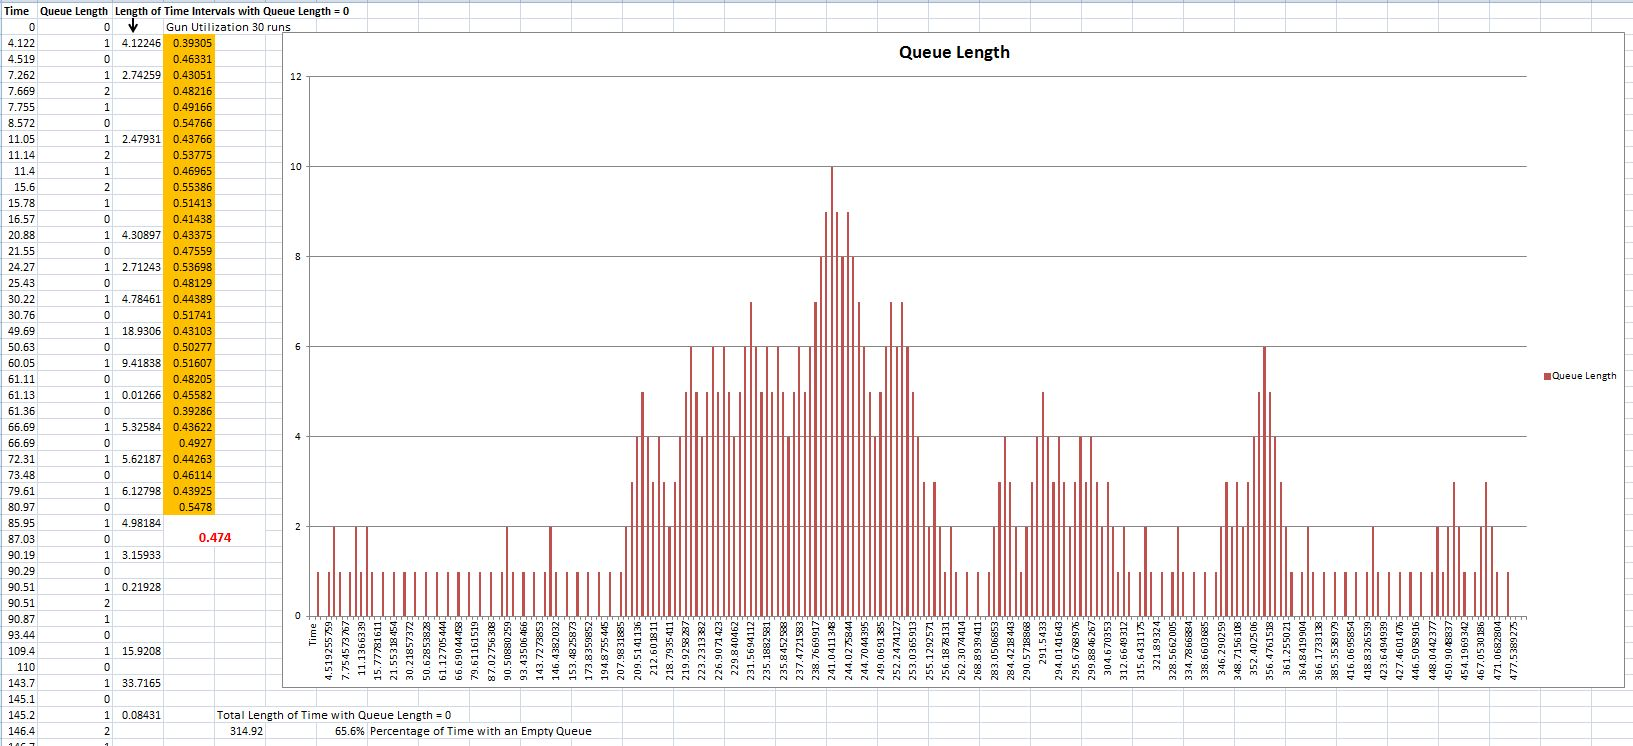
\includegraphics[scale=0.35]{images/requirement3graph.jpg}
	\end{center}
	\caption{Rail gun queue length}
	\label{fig:requirement3graph}
\end{figure}

% Requirement 4 - Is there a warm-up (transient) state for your model?  What metric are you using to identify the transient state?  If the transient state exists, identify approximately when it ends.

The search for a transient state was one of the most interesting aspects of the rail gun investigation performed.  Many graphical inspections of model output were made to try to identify a transient state within the model.  It was our expectation that the transition state would exist and be related to the model starting out at time zero with the queue empty.  It was expected that the initial calls for rail gun support would be more likely to be answered faster due to less delay within the model than during later simulation times.  Ultimately, we could not find any graphical data to support the existence of a transition phase to steady state.  

Our initial focus to identify a transient state was to inspect plots of targets killed versus time (see Figure \ref{fig:requirement4graph} on page \pageref{fig:requirement4graph}).  Graphs inspected step up differently due to the exponential distributions, but the manner the model behaves near time zero is not inconsistent with later behavior.

Additional parameters including targets killed, wait time in the queue, queue length, and wait time at the rail gun were graphically inspected for signs of a warm up phase.  Figure \ref{fig:requirement4graph2} on page \pageref{fig:requirement4graph2} shows a typical graph of these parameters.  Graphical results for each run did vary and there is high unpredictability in the plot parameters, but no clear transient or warm up state could be found. 

\begin{figure}[h!tbp]
	\begin{center}
		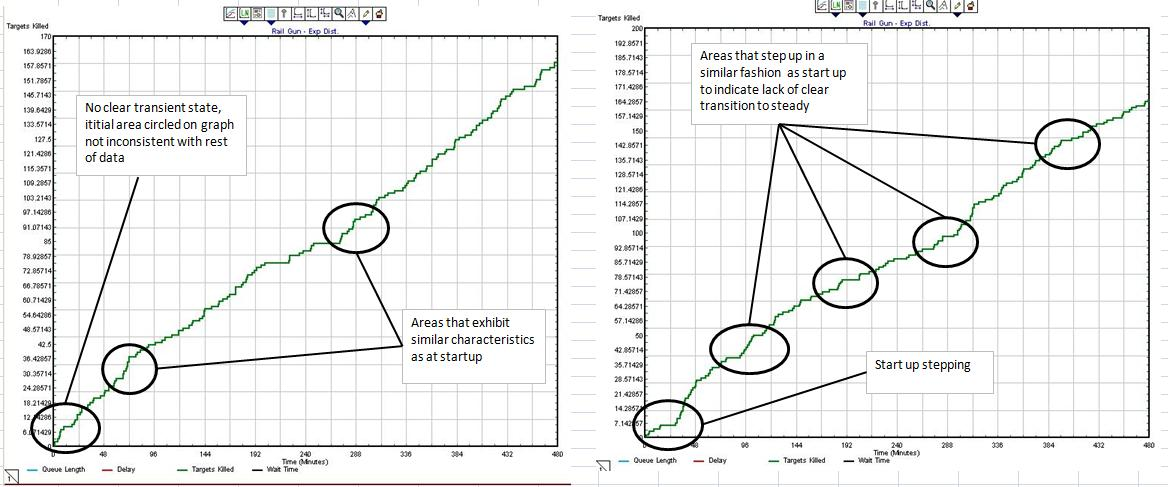
\includegraphics[scale=0.65]{images/requirement4graph2.jpg}
	\end{center}
	\caption{Transition state analysis}
	\label{fig:requirement4graph}
\end{figure}

\begin{figure}[h!tbp]
	\begin{center}
		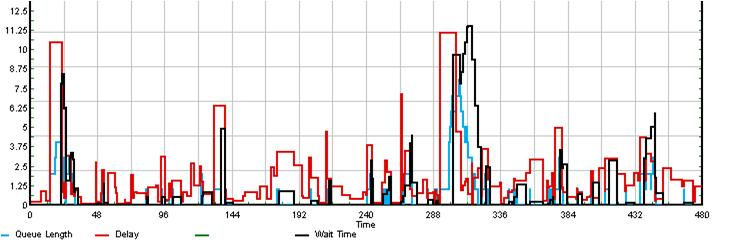
\includegraphics[scale=1]{images/requirement4graph.jpg}
	\end{center}
	\caption{Transition state - additional parameters}
	\label{fig:requirement4graph2}
\end{figure}

% Requirement 5 - On average, how many fire requests at any given time in steady state are waiting for a gun to become available? Provide and interpret a 90% approximate confidence interval for your answer.

We collected statistics from the queue in our ExtendSim rail gun model, paying special attention to the Average Length column, which is the average number of requests in the queue over that simulation run.  Using this data, we get the average number of queue requests waiting for a gun to be 0.454 with CI $(0.405, 0.503)$.

\subsection{Model Conclusions}
% Requirement 6 - Identify at least one other interesting feature of your model�s output.

The delays found within the queue were larger than might be expected for a system that has an average fire request of 3 minutes and only requires 1.5 minutes to prepare, charge, and fire the gun.  Without an understanding of the impact of the use of different types of distributions, one might expect the rail gun to easily stay ahead of the calls for fire support.  However, the average maximum wait in the queue over the 30 simulation runs was 8.47 minutes.   The maximum length of the queue or the maximum number of calls for fire support waiting in the queue had a surprisingly wide range over the 30 simulation runs, with a high of 9 in one simulation, while another had a high of only 3.  The high of 9 led to a 15.77 minute wait in the queue.  The maximum of 3 waiting in the queue led to a 6.13 minute wait period.

These results are directly related to the use of an exponential distribution for both target and fire response times.  The median values of the exponential distribution are lower than the mean values of 3 and 1.5 minutes.  An exponential distribution has a high point that is tangent to the $y-$axis and a smooth curve down to the asymptotic approach to the $x-$axis.  As soon as a cluster of short target inter-arrival times occurs, the rail gun response time would have to match the target cluster to keep up, which is not likely to happen.   Stacking in the queue can also be a result of long inter-response times at the rail gun or a combination of short inter-arrival times and long inter-response times.  A large number of fire calls stacking in the queue or long time delays in the queue indicate combinations of these events have occurred, while lower numbers indicate this rarely occurred during the simulation.
 
When delays occur, an argument can be made that the rail gun loses effectiveness and the expeditionary force will have a difficult time until the rail gun is able to catch up.

% Requirement 7 - Based on your judgment, do you have enough guns on hand?

It is our assessment that when using a single rail gun and exponential distributions for the arrival and server times, that not enough guns are on hand to ensure effective fire support for the expeditionary force.  This assessment is primarily based on our interpretation of the stakeholder time requirements for support, but also influenced by single rail gun utilization, the assumptions made regarding a 100\% kill rate per shot, and the inability of the single gun system to handle a cluster of target arrivals without delays developing.

It is critical to perform stakeholder analysis and investigate the user requirements or expectations for the rail gun system and draw conclusions regarding an acceptable system response time.   The model is constructed with the assumption of an infinite amount of time to respond and still kill a target. This is unrealistic, as long response times would lead to missing killing certain targets, which would put the expeditionary force at risk.  The average maximum wait for the 30 simulation runs in the queue was 10.21 minutes, with one run exhibiting a 15 minute queue delay.  The average maximum delay per run at the rail gun was 8.47 minutes, with the high being over 11 minutes.  Based on known rail gun projectile velocities, a 6 minute flight time is required for the projectile to reach targets at the edge of its 250 mile range.  Data collected from simulations indicates there will be multiple times during a 480 minute time frame where more than 15 minutes would be required from the call for support until the projectile arrived and eliminated the target.   It is our assessment that key rail gun stakeholders would find a 15 minute wait for target elimination to be unacceptable.  The need for quick response time to eliminate targets supports the addition of more guns.   

Utilization data was collected on the rail gun during the model simulations.  It was determined that gun utilization was at approximately 33\%.   In most cases a lower utilization leads to less queuing for customers and means the system is idle more often. This could be considered inefficient, as it is essentially paying for idle time.  An increase in utilization would require more preventive maintenance and downtime due to increased wear and tear on the single rail gun.  This would put the expeditionary force at risk and supports a system with additional guns.  Additional guns would allow maintenance actions to be performed without the system being completely down.  A single point of failure where a sole gun being inoperable puts the expeditionary force at risk should be avoided.

There is a fundamental difference in the rail gun system when compared to other discrete event simulations such as a car wash or a sandwich shop.   In the car wash or sandwich shop simulations, it is beneficial to keep the server busy and not pay for idle time.  There is a balance or trade-off between acceptable customer wait times and server utilization.   For the rail gun case, the stakeholders require the response to be quick.  This results in the idle time of the rail gun crew being a secondary consideration.   The value of infrastructure, base defense, and human lives is weighed extremely high and supports adding a second gun to provide quick and effective support.

\section{Model Variations}
\subsection{Mean Time Between Fire Requests}
% Requirement 8 - When supported forces are in close contact with the enemy, the mean time between fire requests can drop to 45 seconds.  How does that change your answers to (2) to (6)?

The model was modified to change the database table input for fire requests' mean value to 0.75 minutes (45 seconds) from the previous baseline requirement of 3 minutes.  This scenario quickly overwhelms the single rail gun model with no changes to the weapon's operational cycle time parameters for charging, loading, and firing.  A basic trend emerges with the number of targets acquired and killed approximately equal to the number of fire requests built up in the queue at the end of the simulation run's 8 hour duration.

This reduced time holds some interesting implications for our previous findings.
\begin{itemize}
  \item Revised response to requirement 2 - The average time until a target is fired upon is now 118.7 minutes with 90\% confidence interval limits of 115 minutes and 122.3 minutes.
  \item Revised response to requirement 3 - The fraction of the average time until a target is fired upon due to queueing delays is now 0.987.
  \item Revised response to requirement 4 - There is still no observable transient period prior to the commencement of a steady state for this model.  The delay time still exhibits random behavior according to the distribution parameters.  The queue length, wait time and targets killed increase in an approximately linear fashion until the end of the simulation.
  \item Revised response to requirement 5 - On average there are 158.7 fire requests waiting for the rail gun to become available.  The 90\% confidence interval lower and upper limits for this value are 153.7 and 163.6 fire requests.  The simulation will of course provide different outputs over various runs, but in 90\% of the cases - the sample average obtained (158.7), which is our current best parameter estimate for the population mean will be contained within the confidence interval limits.
  \item Revised response to requirement 6 - Two interesting features of the model's output are the gun's near continuous utilization at average 0.99876, and the average maximum wait in the queue of 237.3 minutes.  If the close contact supposition is possible, the utilization would place a premium on an extremely high Mean Time Between Failure (and between preventive maintenance) and an extremely low Mean Time To Repair for the gun.  The average maximum wait time in the queue of nearly 4 hours seems to indicate a low operational effectiveness for the capability in support of ground expeditionary forces achieving mission objectives.
\end{itemize}

% The data collected earlier from our initial ExtendSim models provides a baseline against which we can compare results when we modify the incoming target interval to 45 seconds.  This adjustment yields runs with drastically different statistics over 30 iterations.  Average queue delay is now nearly 2 hours.  There are almost 650 targets generated on average.  By the ends of these 8 hour runs a common result is to have the average engaged almost equal to the amount in the queue.  This situation is clearly overloading the rail gun.  The delay seen now is almost exclusively due to queue delay (over 98\%).  Results are supported and summarized in the graph in Figure \ref{fig:requirement8graph} on page \pageref{fig:requirement8graph} and Table \ref{tab:requirement8table} on page \pageref{tab:requirement8table}.
% 
% \begin{figure}[h!tbp]
% 	\begin{center}
% 		\includegraphics[scale=0.6]{images/Requirement8graph.jpg}
% 	\end{center}
% 	\caption{Results of rail gun model adjusted for 45 second fire requests}
% 	\label{fig:requirement8graph}
% \end{figure}
% 
% \begin{table}[h!tbp]
% 	\begin{center}
% 		\begin{tabular}{l.}
% 			\hline
% 			Avg Queue Wait for All Runs			&		117.2132667 \\
% 			Average Shooter Wait for All Runs	&		1.488266667 \\
% 			Average Total Wait for All Runs		&		118.7015333 \\
% 			\hline
% 			CI Upper	& 122.3435897 \\
% 			CI Lower	& 115.059477 \\
% 			\hline
% 		\end{tabular}
% 	\end{center}
% 	\caption{Results of rail gun model adjusted for 45 second fire requests}
% 	\label{tab:requirement8table}
% \end{table}

\subsection{Keeping Track of Success and Failure}
% Requirement 9 - Based on your judgment, suggest and implement one refinement to this model.  How does your refinement affect your answers to (2) through (6)?  Note, a refinement is not a simple parameter change.

An improvement to our discrete event ExtendSim model was developed (see Figure \ref{fig:requirement9model} on page \pageref{fig:requirement9model}) for a single rail gun system.  Exponential distributions were utilized for all arrival and server (rail gun) times.  In this model, the probability of kill is considered to be 100\% for each round fired. The modifications incorporated into the previous model two $\mbox{Equation}(I)\mbox{\ } (\mbox{Item} > \mbox{Properties})$ functions. This function was used to set, modify, or check on existing items and calculate the desired equations when the item arrives. Additional modifications included a \emph{select item out} function, two separate exit functions (collecting success and failures respectively).

\begin{figure}[h!tbp]
	\begin{center}
		\includegraphics[scale=0.5]{images/Requirement9graph.JPG}
	\end{center}
	\caption{Successes, failures, and utilization}
	\label{fig:requirement9graph}
\end{figure}

The simulation data was pasted from the ExtendSim database into an Excel spreadsheet, where calculations were performed that indicate the average time until a target is fired upon is 3.015 minutes, with a Confidence Interval (CI) of $(2.833, 3.197)$.

Again the fraction of time that is due to queuing delays can be calculated by dividing the average wait in the queue by the average time until a target is fired upon.  Results indicate 50.6\% of the overall time until a target is fired upon is caused by queue delays.  Queue delays are due to the single rail gun being occupied with actions required to fire at earlier target requests.

The delays found within the queue were larger than might be expected for a system that has an average fire request of 3 minutes and only requires 1.5 minutes to prepare, charge, and fire the gun.  There are on average 0.532 fire requests in the queue waiting for the rail gun to become available.  The CI for this result is $(0.466, 0.599)$. The average maximum wait in the queue over the 30 simulation runs was 8.38 minutes.  The queue or the maximum number of calls for fire support waiting in the queue still had a wide range over the 30 simulation runs, with a high of 10 in one simulation, while another had a high of only 3. The median values of the exponential distribution are lower than the mean values of 3 and 1.5 minutes.  

\subsection{Number of Guns vs. Cycle Time}
% Requirement 10 - Would it be better to have one gun with a mean cycle time of 1.5 minutes or four guns with cycle times of 6 minutes?  Why or why not?  Support your assertion with a statistical hypothesis test.

We looked at a number of metrics for distinguishing two conditions, one where we have a single rail gun with a mean cycle time of 1.5 minutes and another where we have four rail guns each of whose cycle times are 6 minutes.  When we approached this analysis we assumed that minimizing queue length would be tantamount to maximizing target acquisition and, hence, would indicate an increase in the likelihood of successful kills on the battlefield.  What we found, however, was that the queue length in both models is relatively short and an analysis of variance (1-way ANOVA) indicates no statistical difference in this metric.

So we looked at other indicators such as average length, average wait, max length, max weight and utilization.  All of these have $p-$values less than $\alpha$ which supports unequal means in these data.  Our findings are summarized below in Table \ref{tab:requirement10} on page \pageref{tab:requirement10}.

\begin{table}[h!tbp]
	\begin{center}
		\begin{tabular}{l.}
			\hline
			\myalign{c}{\textbf{Criteria}} & \myalign{c}{\textbf{$p-$value}} \\
			\hline\hline
			Average Length	& 0.00128 \\
			Maximum Length	& 0.00405 \\
			Average Wait	& 0.0009 \\
			Maximum Wait	& 0.01624 \\
			Queue Length	& \cellcolor{yellow}0.55315 \\
			Utilizaiton		& 0.0 \\
			\hline
		\end{tabular}
	\end{center}
	\caption{Analysis of number of guns vs. cycle time}
	\label{tab:requirement10}
\end{table}

As we can see, the average and maximum wait times are shorter with four rail guns than with one and the data is statistically significant.  Focusing on these criteria, we infer that four guns would result in a faster acquisition and kill time and therefore pose significantly less risk to material damage and human life.
 
\subsection{Normal vs. Exponential Distribution}
% Requirement 11 - This model may be sensitive to the choice of fire request and server distributions.  Set the time between targets to follow a normal distribution with mean 3.0 and standard deviation of 0.25.  Set the gun cycle times to follow a normal distribution with mean 1.5 and standard deviation of 0.5.  How do your answers for (2) to (6) and (9) change?  Explain why using common sense arguments.

The time between call for fire support was changed from an exponential distribution to a normal distribution with mean of 3.0 minutes and standard deviation of 0.25 minutes. The gun cycle time was altered from an exponential distribution to a normal distribution with mean of 1.5 minutes and standard deviation of 0.5 minutes. The modifications resulted in a drastic change in the behavior of the rail gun model, with any queue waiting times being virtually eliminated.

Using 30 simulation runs, the average time until a target is fired upon drops from 2.800 minutes with the exponential distribution to 1.499 minutes with a 90\% CI of $(1.488, 1.511)$ for the normal distribution. The average wait in the queue dropped from 1.310 minutes with the exponential distribution to 0.0009 minutes for the normal. The fractional average of the time until a target is fired upon that is due to queuing delays dropped from 46\% to 0.058\% for the normal distribution. A graphical investigation of plots for targets killed, queue length, rail gun delay, and queue wait time did not reveal a transient state within the normally distributed model.

The standard deviation of the normal distributions plays a critical role in the change in results, as it indicates how widely the time values will vary from the mean. As we know, 3 standard deviations from the mean will account for 99.7\% of the values. The small standard deviation of 0.25 minutes for targets generating a fire request feeds the model in a smoother fashion than the exponential distribution. Even with a larger standard deviation of 0.5 at the rail gun, the model has no problem quickly responding to calls to provide fire support. In 30 runs, the average maximum wait in the queue was 0.12 minutes, as opposed to 10.22 minutes in the exponential distributions.

There are on average 0.00029 fire request in the queue waiting for the rail gun to become available.  The CI for this result is $(0.00015, 0.00042)$.  This large reduction in average queue length compared to the exponential distribution is attributable to the aforementioned relatively small standard deviation values used in this model.  Under this set of assumptions the rail gun deployed as a standalone, single system capability within a battle space or group could be characterized as having a high degree of operational effectiveness.

The exponential distribution is commonly used for waiting time, failure rates, or events where the rate of occurrence remains constant over time. It is important to consider that an exponential distribution has a memory-less property that a normal distribution does not have. This means that the probability of an event occurring at any point in time is the same and independent or not influenced by how long the current wait has been. This feature of exponential distributions contributed to the delays exhibited in the exponential distribution rail gun model.

One other interesting feature of this model's output is the only slightly higher gun utilization rate than for the exponential distribution with same means (0.50022 vs. 0.474 previously).  Whether targets are piling up in the queue or not, \emph{percent busy} is driven by the gun cycle time mainly.  The standard deviation for utilization is also much smaller than it was for 30 exponential runs.

By far the most interesting output feature observed when applying a normal distribution to the refined model with timing-in-the-queue based pass-fail criteria is the disappearance of any failures. The system is now able to keep up with this more controlled variance version of modeling assumptions, and would be deemed an operationally effective capability if only scenarios and CONOPS like this set of assumptions were considered.

\pagebreak
\appendix
\section{ExtendSim Models}
\begin{figure}[h!tbp]
	\begin{center}
		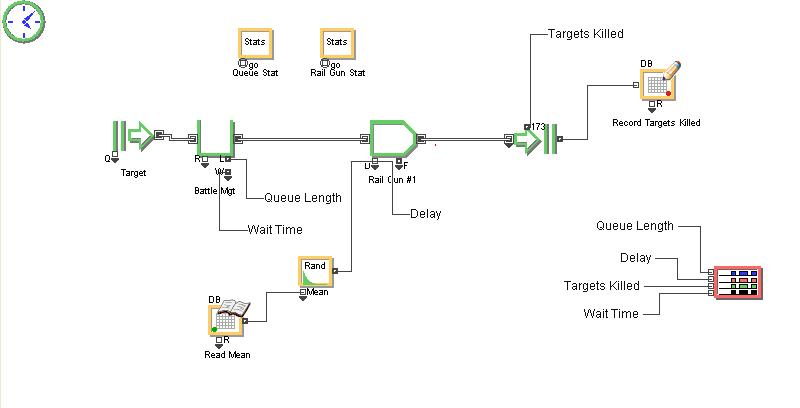
\includegraphics[scale=0.7]{images/requirement1model.jpg}
	\end{center}
	\caption{Discrete event model for single rail gun}
	\label{fig:requirement1model}
\end{figure}

% \begin{figure}[h!tbp]
% 	\begin{center}
% 		\includegraphics[scale=0.5]{images/Requirement8model.jpg}
% 	\end{center}
% 	\caption{Rail gun model adjusted for 45 second fire requests}
% 	\label{fig:requirement8model}
% \end{figure}

\begin{figure}[h!tbp]
	\begin{center}
		\includegraphics[scale=0.5]{images/Requirement9model.JPG}
	\end{center}
	\caption{Rail gun model enhancement showing successes and failures}
	\label{fig:requirement9model}
\end{figure}

\end{document}